\documentclass[border=1pt]{standalone}
\usepackage{tikz}

\newif\ifshowgrid
\showgridtrue          % 改为 \showgridfalse 可去掉像素网格

\begin{document}
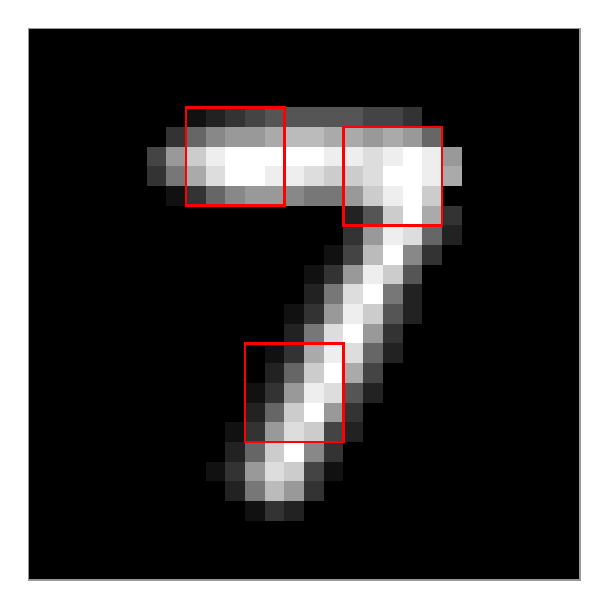
\begin{tikzpicture}[scale=0.25]   % 1 个单位 = 1 个像素

  \fill[black] (0,0) rectangle (28,28);   % 黑底

  % 数字 7 的 28x28 灰度数据（0=黑 ... 15=白），每行 28 个像素
  \foreach \v [count=\n] in {%
    0,0,0,0,0,0,0,0,0,0,0,0,0,0,0,0,0,0,0,0,0,0,0,0,0,0,0,0,% 行1
    0,0,0,0,0,0,0,0,0,0,0,0,0,0,0,0,0,0,0,0,0,0,0,0,0,0,0,0,% 行2
    0,0,0,0,0,0,0,0,0,0,0,0,0,0,0,0,0,0,0,0,0,0,0,0,0,0,0,0,% 行3
    0,0,0,0,0,0,0,0,0,0,0,0,0,0,0,0,0,0,0,0,0,0,0,0,0,0,0,0,% 行4
    0,0,0,0,0,0,0,0,1,2,3,4,5,5,5,5,5,4,4,3,0,0,0,0,0,0,0,0,% 行5
    0,0,0,0,0,0,0,3,6,8,9,9,10,11,11,10,10,9,10,9,6,0,0,0,0,0,0,0,% 行6
    0,0,0,0,0,0,4,9,12,14,15,15,15,15,15,14,14,13,14,15,14,9,0,0,0,0,0,0,% 行7
    0,0,0,0,0,0,3,7,10,13,15,15,14,14,13,12,12,13,15,15,14,10,0,0,0,0,0,0,% 行8
    0,0,0,0,0,0,0,1,3,6,8,9,9,8,7,7,9,12,14,15,12,0,0,0,0,0,0,0,% 行9
    0,0,0,0,0,0,0,0,0,0,0,0,0,0,0,0,2,5,12,15,10,3,0,0,0,0,0,0,% 行10
    0,0,0,0,0,0,0,0,0,0,0,0,0,0,0,0,3,9,14,13,6,2,0,0,0,0,0,0,% 行11
    0,0,0,0,0,0,0,0,0,0,0,0,0,0,0,1,4,11,15,8,3,0,0,0,0,0,0,0,% 行12
    0,0,0,0,0,0,0,0,0,0,0,0,0,0,1,3,9,14,12,5,0,0,0,0,0,0,0,0,% 行13
    0,0,0,0,0,0,0,0,0,0,0,0,0,0,2,7,13,15,7,2,0,0,0,0,0,0,0,0,% 行14
    0,0,0,0,0,0,0,0,0,0,0,0,0,1,3,9,14,12,5,2,0,0,0,0,0,0,0,0,% 行15
    0,0,0,0,0,0,0,0,0,0,0,0,0,2,7,13,15,9,3,0,0,0,0,0,0,0,0,0,% 行16
    0,0,0,0,0,0,0,0,0,0,0,0,1,3,10,14,13,6,2,0,0,0,0,0,0,0,0,0,% 行17
    0,0,0,0,0,0,0,0,0,0,0,0,2,6,12,15,10,4,0,0,0,0,0,0,0,0,0,0,% 行18
    0,0,0,0,0,0,0,0,0,0,0,1,3,9,14,13,5,2,0,0,0,0,0,0,0,0,0,0,% 行19
    0,0,0,0,0,0,0,0,0,0,0,2,6,12,15,9,3,0,0,0,0,0,0,0,0,0,0,0,% 行20
    0,0,0,0,0,0,0,0,0,0,1,3,9,13,12,4,2,0,0,0,0,0,0,0,0,0,0,0,% 行21
    0,0,0,0,0,0,0,0,0,0,2,6,12,15,8,3,0,0,0,0,0,0,0,0,0,0,0,0,% 行22
    0,0,0,0,0,0,0,0,0,1,3,9,13,12,4,1,0,0,0,0,0,0,0,0,0,0,0,0,% 行23
    0,0,0,0,0,0,0,0,0,0,2,7,11,9,3,0,0,0,0,0,0,0,0,0,0,0,0,0,% 行24
    0,0,0,0,0,0,0,0,0,0,0,1,3,2,0,0,0,0,0,0,0,0,0,0,0,0,0,0,% 行25
    0,0,0,0,0,0,0,0,0,0,0,0,0,0,0,0,0,0,0,0,0,0,0,0,0,0,0,0,% 行26
    0,0,0,0,0,0,0,0,0,0,0,0,0,0,0,0,0,0,0,0,0,0,0,0,0,0,0,0,% 行27
    0,0,0,0,0,0,0,0,0,0,0,0,0,0,0,0,0,0,0,0,0,0,0,0,0,0,0,0 % 行28（最后无逗号）
  }{%
    \ifnum\v>0\relax
      \pgfmathtruncatemacro{\col}{int(mod(\n-1,28))}
      \pgfmathtruncatemacro{\ybot}{27-int((\n-1)/28)}
      \pgfmathsetmacro{\gpct}{\v/15}
      \definecolor{px}{gray}{\gpct}
      \fill[px] (\col,\ybot) rectangle (\col+1,\ybot+1);
    \fi
  }

  % 像素网格与边框
  \ifshowgrid
    \draw[gray, opacity=0.4, thin, step=1] (0,0) grid (28,28);
  \fi
  \draw[gray!80, line width=0.6pt] (0,0) rectangle (28,28);

  % ---------- 局部关注框：只看这几处细节就够 ----------
  % 5x5 窗口（对齐像素格）
  \draw[red, line width=1pt] (8,19)  rectangle (13,24);   % 横笔一段
  \draw[red, line width=1pt] (16,18) rectangle (21,23);   % 拐角（横接竖）
  \draw[red, line width=1pt] (11,7)  rectangle (16,12);   % 竖(斜)笔一段
  % 若想用 3x3，把上面三行换成：
%   \draw[red, line width=1pt] (9,20)  rectangle (12,23);
%   \draw[red, line width=1pt] (17,20) rectangle (20,23);
%   \draw[red, line width=1pt] (12,9)  rectangle (15,12);
\end{tikzpicture}
\end{document}